\subsubsection{Paketinis gradientinis nusileidimas}
\label{subsubsec:paklaidos_priklausomybe_paketinis_gradientinis_nusileidimas}

Naudojant paketinį gradientinį nusileidimą su mokymosi greičiu $\eta = 0{,}5$ ir $500$ epochų, paklaida tolygiai mažėja per visą mokymo procesą (žr.~\ref{fig:error_bgd} pav.). Galutinė mokymo paklaida – $0{,}0354$, validavimo – $0{,}0296$. Validavimo paklaida yra mažesnė nei mokymo, o tai rodo, kad modelis nėra persimokęs.

\begin{figure}[H]
    \centering
    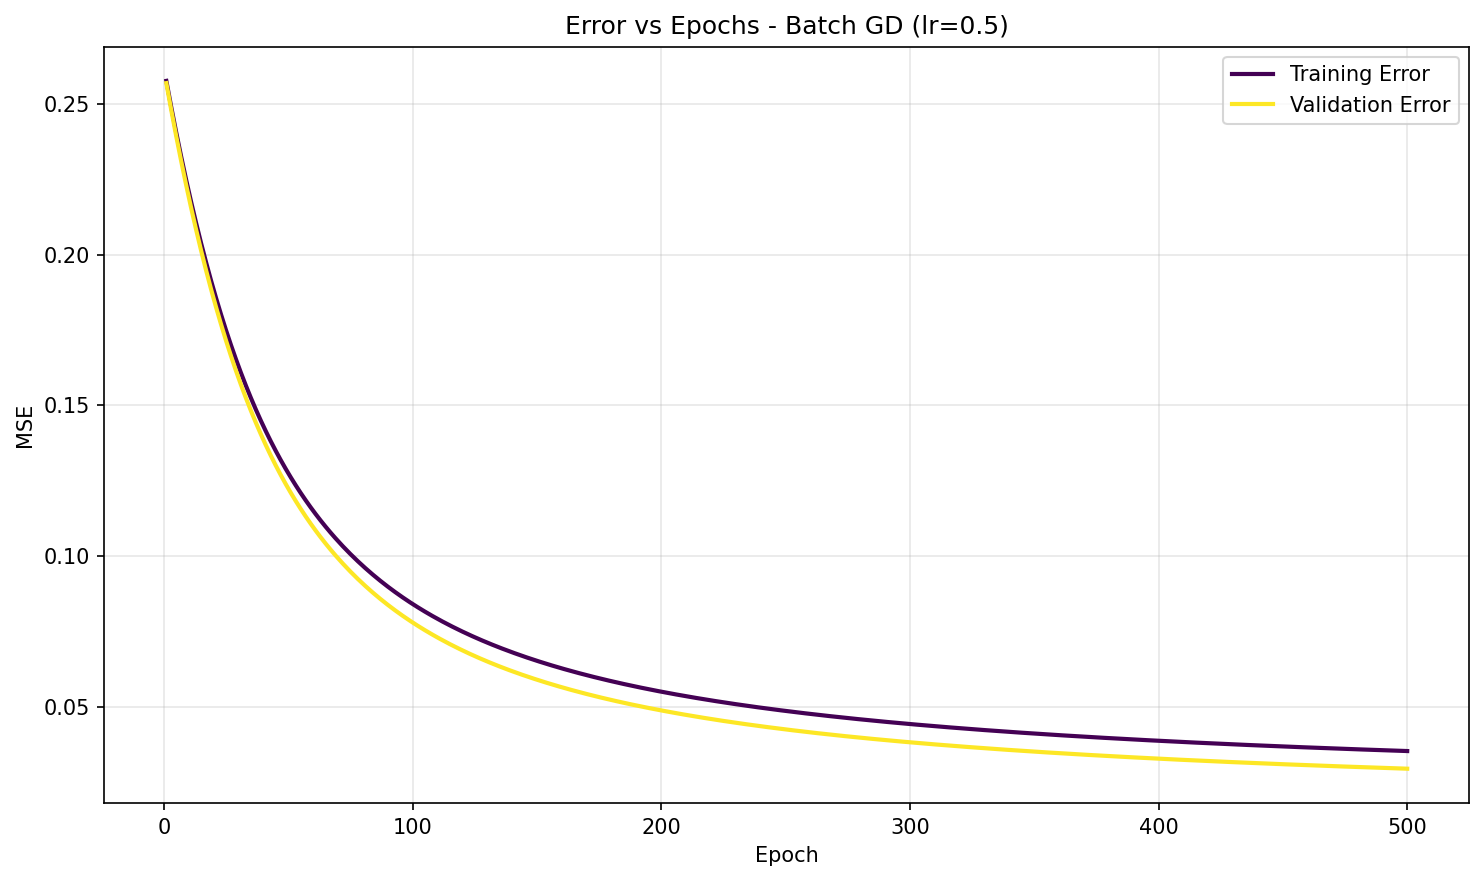
\includegraphics[width=0.85\linewidth]{2Lab/visualizations/error_bgd.png}
    \caption{Paklaidos priklausomybė nuo epochų (paketinis GN, $\eta = 0{,}5$)}
    \label{fig:error_bgd}
\end{figure}